\chapter{Introduction}
\label{ch:introduction}
The current climate crisis necessitates the rapid development of technologies for \ce{CO2} capture. Ideally these technologies should be simple and cheap to deploy. Exploitation of the phenomenon of physical adsorption of \ce{CO2} onto porous materials may comprise a viable solution for both point source and \acrfull{dac}, and \glspl{turbostratic carbon} provides a cheap, simple route to a viable material for such purposes. The following sections provide the essential background of the concepts and applications of the experimental, analytical, and computational work employed in this thesis in order to understand how to develop porosity, measure the developed porosity, and understand the relationship between \ce{CO2} capture and porosity. In addition the author provides for convenience his published review on the modulation of the porosity of carbons for uptake of various gases (\ref{pub:review}) as appendix \ref{ap:review}. This provides much broader information regarding the synthesis of porous carbons outside of just the \glspl{turbostratic carbon} which are examined in this work, methods to measure and control porosity in such materials, as well as the relationship between porosity and uptake of different sorbents in porous carbons. 

\newpage

\section{Synthesis of turbostratic carbons}

\Glspl{turbostratic carbon} are semi-ordered carbonaceous materials characterised as having high surface area due to an extensively porous structure. Gases such as \ce{CO2} can be physisorbed onto the surface of the material making for facile regeneration.\citep{Kuramochi2012Comparative, Ghosh2016} These characteristics make the material attractive for \ce{CO2} capture. In addition, these materials are chemically and thermally robust, meaning that they are suitable for industrial applications.\citep{Kuramochi2012Comparative, Coromina2016, HaffnerStaton2016High} As the only requirement for a material to be suitable for use as a precursor to \gls{turbostratic carbon} is that it have a high carbon content, these materials can be  synthesized  from a  range  of cheap, and even renewable or waste-derived precursors.\citep{Sevilla2014Energy, Sun2017, Titirici2010Chemistry, Blankenship2017Cigarette, Ariharan2018}

The porosity of a carbonaceous material is typically developed \textit{via} a pyrolysis process wherein at first, a semi-graphitic structure is established; the voids between layers forming pores. Pores are then further constructed  \textit{via} intercalation of species between the graphitic layers for example by gases,\citep{Gonzalez2009} or metal ions such as Na or K.\citep{Sevilla2014Energy, Osswald2009Porosity, Wang2012KOH, RuizFernandez2011} Both of these intercalating agents can come from the raw precursor itself or be added to improve pore development. Further pore development comes as the result of chemical reactions, including the oxidation of carbon to form carbonates, or condensing processes including dehydration reactions which form cross-links between graphitic layers.\citep{Sevilla2014Energy, Wang2012KOH, Prahas2008} All of these processes tend to yield pores of a slit-like geometry, whose width is defined by the distance between two adjacent carbon walls, while the other dimensions are not usually defined (or assumed to be infinite).\citep{Sevilla2019, Everett1976Adsorption}

In order to facilitate high levels of porosity development, polymeric carbohydrates and sugars are often hydrothermally carbonised prior to activation with oxidative chemical \glspl{porogen} such as \ce{KOH}, by heating in water under high pressure to form \gls{hydrochar}. \Gls{hydrochar} is a low-surface area material (\qty{\sim30}{\metre\squared\per\gram}) composed of microspheres with hydrophilic reactive oxygen moieties at the surface. The overall overall oxygen concentration of the material is also increased relative to that of the precursor.\citep{Titirici2010Chemistry, Sevilla2011High} Dried \gls{hydrochar} is then more susceptible to \ce{KOH}-activation due to the improved reactivity between K and the oxygen-rich outer layer of the material.\citep{Sevilla2011High, Sevilla2009Chemical} In some cases, \gls{htc} forms a necessary step in the activation of a precursor, as some carbohydrates will not activate unless they have been first hydrothermally carbonised.\citep{Ares2014}

The following subsections detail background and rationale for the synthesis routes towards \glspl{turbostratic carbon} employed in this thesis.

\subsection{From Cigarette Butts}

\acrfullpl{ucb} pose a large environmental hazard as a result of (i) being made of non-biodegradable \acrfull{ca} as well as (ii) containing a myriad of toxic chemicals.\citep{Slaughter2011, Puls2011, chevalier2018nano} As they are the most common waste material worldwide, there have been attempts to reduce their environmental presence, initially \textit{via} anti-littering campaigns.\citep{Prevention2011, Harris2011} More promising however is the prospect of valorising \acrshortpl{ucb} by various means, including conversion to activated carbons as reported by the author in \ref{pub:CB} as well as many other researchers - a summary of preparation conditions and properties of resultant \glspl{turbostratic carbon} is given in table \ref{tb:cb_carbons_lit}.\citep{Soltani, Soltani2013, lima2018, xiong2019nitrogen, Lee2014, Hamzah2017, Yu2018, Wang2016a, Koochaki2019, Bilge2019}

\afterpage{
    \begin{landscape}
    \begingroup
    \renewcommand{\arraystretch}{1.2}
    %\setlength{\tabcolsep}{10pt}
    \vspace{-16.71507pt}
    \begin{table}[hptb]
        \centering
        \caption{Details of preparation, activation conditions, porosity and composition of selected \acrshort{ucb}-derived \glspl{turbostratic carbon} reported in the literature. For simplicity, any materials derived using a non-inert atmosphere\citep{Lee2014} or \textit{via} microwave activation\citep{Hamzah2017} are excluded. For the porogen, number in brackets indicates the mass ratio, if reported. The number in brackets following the BET area, $A_{BET}$ is the micropore surface area, where reported. The average pore width, $w_{avg}$ is taken as reported without any further analysis. O/C ratio is the atomic ratio. }
        \label{tb:cb_carbons_lit}
        \begin{tabularx}{1.8\textheight}{p{70mm}llrlllll}%p{70mm}llrllllp{10mm}}%{llllll}
            \toprule
                \textbf{Preparation} & \multicolumn{2}{c}{\textbf{Pyrolysis}} & \multicolumn{2}{c}{$\mathbf{A_{BET}}\ $ \textbf{/ \unit[detect-weight]{\meter\squared\per\gram}}} & $\mathbf{w_{avg}}\ $ \textbf{/ \unit[detect-weight]{\angstrom}} & \textbf{O/C} &  \textbf{Elements} & \textbf{Ref.}\\ 
                & $\mathbf{T\ /\ ^{\circ}C}$ & \textbf{\Gls{porogen}} & & & \\
            \midrule
                - & 900 & KOH (1) & 224 & & 32 & 0.34 & K, Na, Si, Cl, Ti & \citep{Soltani} \\
                - & 900 & - & 637 & & 33 & 0.085 & Si, K, Ti & \citep{Yazdi2012} \\
                %\Gls{htc} followed by \ce{NaOH_{(aq)}} impregnation & 190 & \ce{NaOH} (0.4) & - & & - & &  & \citep{lima2018} \\
                Formation of polypyrrole composite & 800 & KOH (1.5) & 3420 & & 46 & 0.12 & & \citep{Xiong2018a} \\
                - & 900 & - & 573 & (395) & 25 & & Ti, N & \citep{Lee2014} \\
                %Cut into pieces & 800 & - & 1285 & & <120 & 0.029 & N & \citep{Yu2018} \\
                Soaked in \ce{NH4VO3_{(aq)}} then dried. Heated to \qty{270}{\degreeCelsius} in a \ce{NH3}/\ce{N2} atmosphere & 800 & - & 164 & & >100 & & & \citep{Wang2016a} \\ 
                Soaked in \ce{NaOH_{(aq)}} (\qty{48}{\volpercent}), then carbonised at \qty{400}{\degreeCelsius} & 800 & NaOH & 1083 &  & 22 & 0.23 & Na & \citep{Koochaki2019} \\
                - & 800 & - & 571 &  & 27 & 0.29 & & \citep{Koochaki2019} \\
                - & 800 & - & 262 & & 45 & & & \citep{polarz2002hierachical} \\
                Washed in ethanol and water, carbonised at \qty{600}{\degreeCelsius} & 800 & \ce{KOH} (5) & 2751 & & <20 & & & \citep{Sun2017} \\
                \Gls{htc} & 600 & \ce{KOH} (4) & 4310 & (3867) & <20 & 0.53 & N & \citep{Blankenship2017Cigarette} \\
                \Gls{htc} & 800 & \ce{KOH} (4) & 1012 & & & & & \citep{Bilge2019} \\
            \bottomrule
        \end{tabularx}%
    \end{table}
    \endgroup
    \end{landscape}
}

\begin{sloppypar}
The reported porosity of carbons derived from \acrshortpl{ucb} is highly varied depending on synthetic conditions - see table \ref{tb:cb_carbons_lit}. In the absence of an \gls{activating agent}, and without pre-carbonisation steps, $A_{BET}$ typically does not exceed \qty{700}{\metre\squared\per\gram}.\citep{Koochaki2019, Soltani2013, Yazdi2012, Lee2014, Hamzah2017} Whereas using a \gls{porogen}, and/or pre-carbonising in air or hydothermally can improve surface areas to around \qty{3000}{\metre\squared\per\gram}.\citep{Xiong2018a, Koochaki2019, Sun2017, Bilge2019} The author's reports of ultrahigh porosity from KOH-activated hydrothermally carbonised \acrshortpl{ucb} in \ref{pub:CB} (BET surface area ($A_{BET}$) \qty{>4000}{\metre\squared\per\gram}, pore volume \qty{>2.00}{\cm\cubed\per\gram}) and high degree of microporosity (\qty{>90}{\percent}) are partially corroborated by the similar results using hydrochar derived from pure \acrshort{ca} in \ref{pub:CA}, suggesting that \acrshort{ca} is an ideal precursor for activation to yield high surface area carbons. The structure of \acrshort{ca} (see figure \ref{fig:cellulose_acetate}) - especially the labile acetyl groups - is likely a large contributor to the high porosities reported in derived activated carbons. Xiong \textit{et al.} also report a nitrogen-doped \acrshort{ucb}-derived activated carbon with hierarchical porosity and $A_{BET}$ of \qty{3420}{\metre\squared\per\gram}, though this result is dubious as (i) the \ce{N2} isotherm does not include ultralow pressure data, (ii) freespace appears to be incorrectly measured and (iii) isotherm measurement is not described in the text.\citep{xiong2019nitrogen} It was suggested in \ref{pub:CB} that the unusually high porosity of \acrshort{ucb}-derived carbons may be contributed to by the action of so-called contaminant-\glspl{porogen}, i.e. trace elements found in cigarette butts that can act as \glspl{activating agent} because carbons from \acrshortpl{ucb} had greater porosity than unused, i.e. `fresh' \acrshortpl{cb}. However, another factor may be the specific treatment of the \acrshortpl{ucb} prior to any carbonisation - that is the removal of any paper, residual ash and tobacco.
\end{sloppypar}


\begin{figure}[ht!]
    \centering
    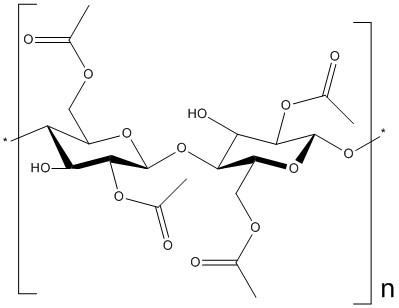
\includegraphics[width=0.7\columnwidth, keepaspectratio]{4-cbs/figs/cellulose_acetate.jpg}
    \caption{Structure of cellulose acetate.}
    \label{fig:cellulose_acetate}
\end{figure}

The trace element composition of \acrshortpl{ucb} has been studied by various means, including neutron activation analysis of the intact butts,\citep{iskander1992multielement, Iskander1985, jenkins1985neutron, Wu1997} \gls{adsorption} and emission spectroscopy of various aqueous extracts,\citep{MussaloRauhamaa1986, Kazi2009, Moriwaki2009, Moerman2011, Pelit2013, Dobaradaran2018} voltammetry experiments,\citep{Nitsch1991, Kalcher1993} and mixed methods according to environmental contaminant quantification standards.\citep{cardoso2018exposure} The reported concentrations of different elements in \acrshortpl{ucb} has a great degree of variability depending on collection site, method, and brand. For example, work by Iskander \textit{et al.} indicates that \ce{Al} can be present in concentrations as low as \num{59}, and as high as \qty{2200}{\micro\gram\per\gram}, depending on the country of origin of the smoked cigarette butt. Similarly, \acrshort{ucb} samples collected from the environment\citep{Dobaradaran2017, Moriwaki2009, Moerman2011, chevalier2018nano} may have lower quantities of some elements due to leaching, but simultaneously may absorb some elements from the environment (for example from sea water). Trace elements have been identified in \acrshortpl{ucb} from almost every region of the periodic table, including alkali and alkaline earth metals;\cite{MussaloRauhamaa1986, Iskander1985, iskander1992multielement, jenkins1985neutron, Wu1997, cardoso2018exposure}  transition metals, post transition metals and metalloids;\citep{MussaloRauhamaa1986, Dobaradaran2017, Iskander1985, jenkins1985neutron, Wu1997, Moriwaki2009, Moerman2011, Pelit2013, Dobaradaran2018, Ren2017, cardoso2018exposure, chevalier2018nano} lanthanides;\citep{iskander1992multielement} and halogens.\citep{Iskander1985, iskander1992multielement, jenkins1985neutron, Wu1997} Cigarette butt derived carbons have been also been found to contain various metals in trace quantities (see table \ref{tb:cb_carbons_lit},\citep{Soltani, Soltani2013, Yazdi2012} although \ce{Ti}, \ce{K}, and \ce{Na} have also been reported at quantities above \qty{1}{\wtpercent}.\citep{Soltani, Soltani2013, Yazdi2012, lima2018, Lee2014} In addition the presence of \ce{Ca}, \ce{K}, \ce{Mg}, \ce{Na}, and \ce{Al} were identified in \acrshort{ucb}-derived \gls{hydrochar} reported in \ref{pub:CB}.

\subsection{Impregnation Methods}

Most commonly in the synthesis of activated carbons \glspl{porogen} are added to precursors by physical mixing with the precursor - i.e. some combination of grinding and stirring.\citep{Aljumialy2020Porous, Blankenship2017Cigarette, Altwala2020Predictable, Sevilla2016Highly} An alternative technique is to impregnate the precursor with a (typically aqeuous) solution of \gls{porogen}.\citep{Botome2017Preparation, Ge2019Highly, Adlak2021Physicochemical, Shi2021Copper, Han2021Mulch} While there is scant evidence that solution impregnation has better outcomes over physical mixing in terms of porosity development, the rationale of the former technique is that the \gls{activating agent} will be more evenly distributed throughout the precursor thus providing more homogenous porosity in the product however there is as yet no study to support this. 

A further method using oxidative chemical activation is so-called organic salt carbonisation wherein the metal cation of an organic salt activates the carbonised precursor during pyrolysis. Reports, in particular from Sevilla \textit{et al.} show that this method allows for a high degree of tunability in carbon PSDs by changing the identity of the activating cation.\citep{Sevilla2013general, Tsumura2014Structure, Ferrero2015Mesoporous, Ferrero2016Efficient, Fuertes2015Hierarchical, Roberts2015Hierarchically, Yadav20123D, Yang2018Spontaneous} The majority of anions used in organic salt carbonisation are small molecules such as gluconate or citrate,\citep{Sevilla2013general, Yang2017Template, Sevilla2014Direct, Tsumura2014Structure, Ferrero2015Mesoporous, Ferrero2016Efficient, Fuertes2015Hierarchical, Yang2020Production, Fuertes2014One} however polymers have also been employed.\citep{Puthusseri20143D, Roberts2015Hierarchically, Yadav20123D, Hines2004Surface} 

The philosophy of these two emergent techniques (solution impregnation and organic salt carbonisation) for porogen-precursor mixing is that (i) the process can be simplified, (ii) porosity can be more readily controlled, and (iii) porosity is more homogeneous throughout the product. These effects are supposedly a result of both improved \gls{porogen}-precursor contact, and more homogeneous \gls{porogen} distribution. For the purposes of this work, mixing techniques with such goals are collectively termed `impregnation' methods. In terms of solution impregnation, thus far syntheses have only been reported wherein the precursor is mixed with the \gls{porogen} directly prior to pyrolysis.\citep{Botome2017Preparation, Ge2019Highly, Adlak2021Physicochemical, Shi2021Copper, Han2021Mulch, Boujibar2018CO2} That is, it has not been attempted to impregnate the \gls{porogen} at the \gls{htc} step. The observation made by Zhang \textit{et al.} that the formation of \ce{K} salts with oxygen-rich moieties on the surface of calcined glucose is associated with improvements in ultramicroporosity,\citep{Zhang2019situ} is notable and provides scope for further control over porosity in \glspl{turbostratic carbon}.

On the other hand, while the porosity of carbons derived through organic salt carbonisation has been exploited through changing the cation,\citep{Sevilla2013general, Tsumura2014Structure, Ferrero2015Mesoporous, Ferrero2016Efficient, Fuertes2015Hierarchical, Roberts2015Hierarchically, Yadav20123D, Yang2018Spontaneous} the capacity for more precise control over porosity by changing the degree of substitution of a cation on a polymer chain has not yet been explored. In studies using physical mixing, the \gls{porogen}:precursor weight ratio is typically reported.\citep{Altwala2020Predictable, Adeniran2015Compactivation, Blankenship2017Cigarette, Sevilla2016green, Ludwinowicz2015Potassium, Deng2015Inspired, Alhamed2015Preparation, Hu2003simple} Oxidative chemical activation primarily relies on redox reactions between \ce{C} and the \gls{porogen}, thus knowing the exact stoichiometric  \gls{porogen}:\ce{C} ratio may provide a route to understanding the precise effects of \gls{porogen} concentration on carbon porosity.


\section{Physisorption \& porosity}
\label{s:adsorption_porosity}
Porous materials possess an interconnected pore system where pores are defined as voids which are deeper than they are wide.\citep{mcnaught1997compendium, Thommes2015Physisorption} Additionally, pores are defined as being able to contain fluid, which indirectly gives a minimum width for voids to be considered pores of \qty{2.6}{\angstrom}, as this is the kinetic diameter of the smallest practical fluid specie, \ce{He}.\citep{Thommes2015Physisorption, Lide2007Handbook} The ability of porous materials to contain fluids has led to the use of the phenomenon of adsorption being used to characterise their porosity. That is, knowledge of the behaviour of the system when the material is enriched with a fluid is utilised to understand pore size, shape and interconnectivity. In particular, so-called \gls{physisorption} is exploited wherein \gls{adsorbate}-\gls{adsorbent} interactions do not include any sort of chemical attraction but instead rely on non-bonding forces\citep{Thommes2015Physisorption} - thus hypothetically (although not always in practice), structure ought not be significantly conflated with surface chemistry. What follows is a discussion of the various types of pore structures and associated adsorption phenomena, and thus an overview of methods to determine porosity from an isotherm.

\subsection{Pore characteristics and filling mechanisms}
\label{ss:pore_filling}

The \acrfull{iupac} defines ranges of pore sizes according to the mechanisms of pore filling by an \gls{adsorbate}.\citep{Thommes2015Physisorption} The three main mechanisms; \gls{micropore} filing; monolayer adsorption; and multilayer adsorption are illustrated in figure \ref{fig:filling}. Specifically, \glspl{micropore} (\qty{<20}{\angstrom})\citep{mcnaught1997compendium} are filled at ultralow relative pressures, and are characterised by strong heats of adsorption due to complementary \gls{adsorbate}-\gls{adsorbent} interactions from all pore walls.\citep{dubinin1989fundamentals} The subdivision into \glspl{ultramicropore} (\qty{<7}{\angstrom}) and \glspl{supermicropore} (\qtyrange[range-units=single]{7}{20}{\angstrom})\citep{mcnaught1997compendium} is derived from the fact that pores narrower than \qty{7}{\angstrom} can fit two adjacent rows of \ce{N2} molecules,\citep{Thommes2015Physisorption} and thus have the highest degree of pore wall potential overlap. \Glspl{mesopore} (\qtyrange[range-units=single]{20}{500}{\angstrom})\citep{mcnaught1997compendium} are characterised by being large enough to allow monolayer adsorption. That is, all adsorbed molecules are in contact with the surface and are not significantly influenced by attraction to the adjacent or opposite pore wall.\citep{gregg1967adsorption, yang1997gas} As pressure increases, repulsive \gls{adsorbate}-\gls{adsorbate} interactions are overcome so that additional \gls{adsorbate} molecules adsorb on top of the monolayer - this process is known as multilayer adsorption. The widest pore size classification is \glspl{macropore} which are larger than 500 \unit{\angstrom}\citep{mcnaught1997compendium} and are not easily characterised by isothermal gas adsorption experiments, instead necessitating the use of mercury intrusion porosimetry for determination of porosity.\citep{abell1999mercury, gregg1967adsorption, haynes1973pore} In addition to these principal adsorption processes, in \glspl{mesopore} capillary condensation can occur at relative pressures greater than \num{\sim0.2} wherein the adsorbate enters a liquid-like state despite being below saturation pressure. This can lead to hysteresis in the resultant isotherm\citep{Thommes2015Physisorption, monson2012understanding} which is discussed in more depth in section \ref{ss:iso_interpretation}.

\begin{figure}[t!]
    \centering
    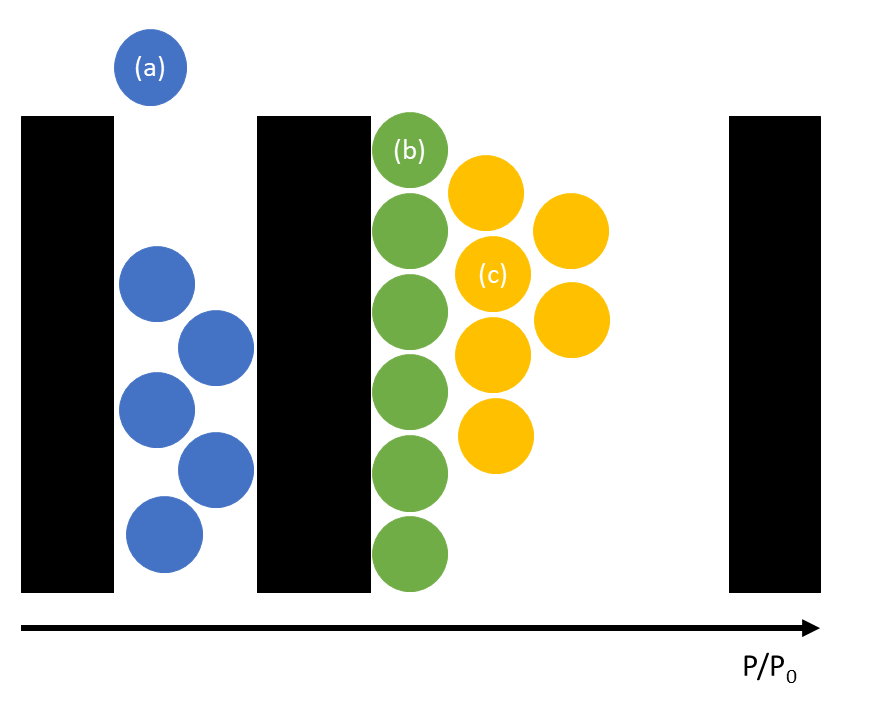
\includegraphics[width=\columnwidth, keepaspectratio]{1-introduction/figs/pore_filling.png}
    \caption{The three principle pore filling mechanisms, in order of their occurence with increasing relative pressure; (a) micropore filling; (b) completion of the monlayer in mesopores; and (c) multilayer adsorption.}
    \label{fig:filling}
\end{figure}

While few materials show uniform pore shape, idealised shape is defined by \acrshort{iupac} according to five characteristic shapes; cylindrical, slit, funnel, sphere, and ink-bottle.\citep{rouquerol1994recommendations, kaneko1994determination, zdravkov2007pore} For example while aluminium oxides typically have cylindrical pores,\citep{zdravkov2007pore} \glspl{turbostratic carbon} are usually assumed to have slit-shaped pores,\citep{Everett1976Adsorption, Jagiello20132D, Lastoskie1993} although carbide-derived carbons have been shown to possess cylindrical or spherical pores.\citep{kurig2016suitability} Zeolites have a broad range of pore shapes.\citep{park2002effect} 

\begin{figure}[b!]
    \centering
    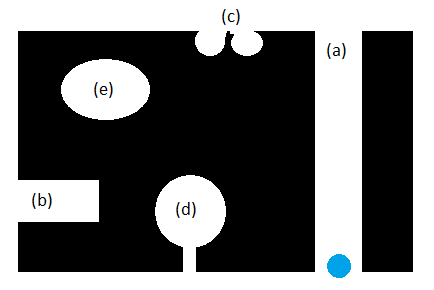
\includegraphics[width=\columnwidth, keepaspectratio]{1-introduction/figs/pore_accessibility.png}
    \caption{The different types of pores classified according to their accessibility; (a) an open, through pore; (b) an open, blind pore; (c) external pores; (d) a chemically closed pore; and (e) a closed pore. The small blue dot indicates the probe molecule size.}
    \label{fig:pore_accessibility}
\end{figure}

In addition to shape and size, pores are also defined by their degree of accessibility. Figure \ref{fig:pore_accessibility} illustrates this type of pore classification. In general, pores can be termed as `closed' or `open', based on whether or not they have an accessible entrance. In the case of open pores, these are further subdivided into `through' pores wherein both ends of the pore are accessible, and `blind' pores wherein only one end of the pore is accessible. In addition, porosity can be formed through undulations on the surface, provided that the depth of these undulations is greater than the width. These are known as `external pores'. However open pores are not necessarily accessible to an adsorptive, that is there entrance may be smaller than the adsorptive molecule - these pores are termed as `chemically closed'. This can occur for ink-bottle pores with a narrow neck, or for very narrow slit or cylindrical pores.\citep{rouquerol1994recommendations, kaneko1994determination, zdravkov2007pore} Porosimetry is only able to quantify apparent porosity as defined by `true' open pores (i.e. not chemically closed) and indeed for gravimetric adsorption applications this is the the only kind of meaningful porosity. However, closed pores nonetheless contribute to a materials bulk density and thus can influence \textit{volumetric} uptake capacity for an adsorptive.


The final characteristic of porous structures is porosity hierarchy. Materials like \acrshortpl{mof} and zeolites typically possess uniform or unimodal porosity,\citep{WeitkampZeolites, Siriwardane2005Adsorption, Ding2019Carbon, lin2009hydrogen} whereas \glspl{turbostratic carbon} typically have multiple- or even a continuous range of (i.e. hierarchical) pore widths.\citep{Li2020Hierarchical, Sevilla2014Energy, Xia2008Hierarchical, Balahmar2017Biomass} The pore hierarchy or lack thereof can play an important role in which applications the material is best suited to - for example a uniform \acrfull{psd} can be used to exclude molecules above a certain size.\citep{qian2020mof, reid2001adsorption, Adeniran2014family}

\subsection{Isotherm classification and interpretation}
\label{ss:iso_interpretation}

The various adsorption behaviours of a porous material discussed in the previous section result in distinct and interpretable forms of the resultant isotherms. As a general rule, the relative amount of gas adsorbed in different pressure ranges gives an indication of the amount of porosity in the internal \gls{micropore} and \gls{mesopore} regions as well as the amount of external surface area. To demonstrate, a labelled isotherm is shown in figure \ref{fig:isotherm_anatomy}. High adsorption in the low pressure region indicates the presence of \glspl{micropore}, while an increase in uptake at pressures around the midpoint of the isotherm indicate mesoporosity. If there is a plateau in the middle of the isotherm, this typically indicates that a monolayer has formed. The curvature of the isotherm prior to the plateau (the adsorption `knee') is indicative of the breadth of the \acrshort{psd}; a gentle knee shows a broad \acrshort{psd}, while a sharp knee indicates that pore sizes are narrowly distributed. Finally, high uptake as relative pressure approaches 1 is indicative of adsorption on the external surface, showing that the material is non-porous or macroporous.\citep{Thommes2015Physisorption} \acrshort{iupac} has designated eight distinct isotherm types.\citep{Thommes2015Physisorption, Sing1985} These need not be discussed in full detail here - it is sufficient to state that types I(a) and (b) isotherms are indicative of microporosity, while IV(a), IV(b) and V are seen on isotherms with high mesoporosity. Nonporous samples typically exhibit type II, III or VI isotherms. The variation in shapes can be indicative of surface chemistry and/or pore size hierarchy.\citep{thommes2014physical, monson2012understanding} Of course as a lot of materials exhibit multiple types of porosity, many materials exhibit characteristics of multiple isotherm types.\citep{Thommes2015Physisorption} 

\begin{figure}[t!]
    \centering
    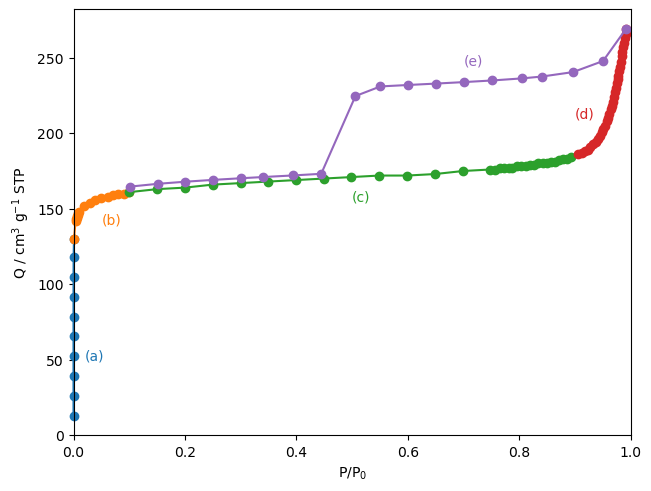
\includegraphics[width=\columnwidth, keepaspectratio]{1-introduction/figs/isotherm_anatomy.png}
    \caption{An isotherm of \ce{N2} on a turbostratic carbon. The isotherm possesses (a) high uptake in the micropore region, indicating microporosity; (b) a sharp knee due to a narrow \acrshort{psd}; (c) a plateau in the medium pressure region due to formation of a monolayer this remains flat in the middle of the isotherm due to lack of mesoporosity; (d) high uptake as relative pressure approaches 1 showing external surface adsorption; and (e) a hysteresis loop due to capillary condensation.}
    \label{fig:isotherm_anatomy}
\end{figure}

Apart from the general isotherm types, the presence of hysteresis - i.e. desorption releasing less \gls{adsorbate} than is taken up during adsorption at an identical relative pressure - is indicative of capillary condensation.\citep{thommes2014physical, monson2012understanding, landers2013density} As with characteristic isotherm types, \acrshort{iupac} has defined six distinct forms of hysteresis loop. Depending on the type of hysteresis loop, its presence may indicate adsorption metastability in an `open' pore, pore network effects and/or other forms of pore blocking.\citep{Thommes2015Physisorption} Each of the six hysteresis loops are associated with specific kinds of materials - for example H4 loops are frequently found in micro-mesoporous carbons, whereas H1 is typically associated with materials possessing uniform open mesopores.\citep{Thommes2015Physisorption, monson2012understanding}  

\subsection{Isotherm models}

The theory of adsorption on a surface can be described mathematically, that is loading of \gls{adsorbate} on an \gls{adsorbent}, $Q$ can be described as a function of pressure, $P$. In the simplest instance, Henry's law\citep{henry1803experiments} (equation \ref{eq:henry}) describes a linear increase in $Q$ with increasing $P$.

\begin{equation}\label{eq:henry}
    Q(P) = K_H P
\end{equation}

Of course, a linear relationship is unrealistic as saturation eventually occurs. Nonetheless the Henry constant, $K_H$ an be used as an approximation of the strength of interaction between \gls{adsorbate} and \gls{adsorbent}. Improvements can be attained through treating the isotherm as a quadratic or virial function, or by the Freundlich approach which modifies the Henry equation to account for the unavailability of adsorption sites by with increase in loading by using the exponent $\frac{1}{m}$, but this still does not account for saturation. Furthermore, neither of these approaches consider the specific case of adsorption of gases onto solid surfaces, instead being more suited to absorption of gas into a liquid. Such a theory was first introduced by Langmuir using kinetics. This assumes a reversible reaction between an ideal \gls{adsorbate}, $A_g$ and an \gls{adsorption} site, $S$ to form the adsorbed complex, $A_{ad}$. The reaction proceeds until it reaches equilibrium with constant $K$;

\begin{equation}
    \ce{A_g + S <=>[K] A_{ad}}
\end{equation}

From this can be derived the Langmuir isotherm (equation \ref{eq:langmuir}), which also accounts for the formation of the monolayer which under this theory is the maximum possible loading, by including the monolayer capacity, $Q_m$.

\begin{equation}\label{eq:langmuir}
    Q(P) = Q_m \frac{K P}{1 + K P}
\end{equation}

This can then be adapted to account for \gls{adsorbent} heterogeneity by considering multiple \gls{adsorption} sites, each with their own equilibrium constants, $K_i$ and monolayer capacities $Q_{m_i}$. Thus the isotherm is modelled as a summation of Langmuir isotherms as in equation \ref{eq:multi_langmuir}. Alternatively, as in the T\'{o}th model, a heteroegeneity factor, $t$ can be used - see equation \ref{eq:toth}. 

\begin{equation}\label{eq:multi_langmuir}
    Q(P) = \sum_{1} Q_{m_i} \frac{K_i P}{1 + K_i P}
\end{equation}

\begin{equation}\label{eq:toth}
    Q(P) = Q_m \frac{K P}{\sqrt[t]{1 + (K P)^t}}
\end{equation}

Thus, surface heterogeneity can be quantified by $t$ (equation \ref{eq:toth}) or the number of adsorption sites (equation \ref{eq:multi_langmuir}). In addition, it has been recently shown that equilibrium constant(s) can be use to approximate the potential energy of adsorption, $\varepsilon$ as a function of surface coverage (i.e. fractional loading).\citep{whittaker2013predicting} On the other hand, the  Dubinin-Radushkevitch and later the Dubinin-Astakhov (see equation \ref{eq:da}) models explicitly considers the thermodynamics of adsorption and so $\varepsilon$ is included in such a treatment.

\begin{equation}\label{eq:da}
    Q(P) = Q_m \exp{ \left[ - \left( \frac{ -R T \ln{\left( \frac{P}{P_0}\right)}}{\varepsilon} \right) \right]^m }
\end{equation}

What is lacking in all of the models discussed above is a description of multilayer adsorption. Stephen Brunauer, Paul Emmet, and Edward Teller expanded Langmuir theory to account for multilayer \gls{adsorption}, which occurs at higher pressures and temperatures. The following assumptions are made;\citep{Brunauer1938Adsorption}

	\begin{enumerate}[label=(\arabic*)]
		\item Gas molecules adsorb on solid layers infinitely,
		\item Gas molecules only interact with adjacent layers,
		\item The Langmuir theory can be applied to each layer,
		\item The enthalpy of \gls{adsorption} for the first layer is constant and greater than that for subsequent layers,
		\item After monolayer \gls{adsorption}, the enthalpy of \gls{adsorption} is the same as that of liquefaction.
	\end{enumerate}

The total quantity of gas adsorbed, $Q$  and thus the proportional surface coverage, $\theta$ is related the quantity of the monolayer, $Q_m$ by equation \ref{eq:bet}. This contains the constant $c$ which describes (see equation \ref{eq:bet_c}) the difference in heats of adsorption, $\lambda$ between the first and subsequent layers. The latter is assumed to be the heat of liquefaction $\lambda_L$.

\begin{equation}\label{eq:bet}
    \theta(P) = \frac{Q}{Q_m} =  Q_m \frac{c P}{\left( 1 - \frac{Q}{Q_0} \right) \left(P_0 + P \left(c - 1 \right) \right)}
\end{equation}

\begin{equation}\label{eq:bet_c}
    c = \exp{\frac{\lambda_1 - \lambda_L}{RT}}
\end{equation}

Equation \ref{eq:bet} can be rearranged to give equation \ref{eq:bet_plot}, which yields a linear relationship. When applied to an iostherm both the thermodynamic constant $c$ and the monolayer loading, $Q_m$ can be derived. From the former the enthalpy of monolayer adsorption can be calculated. The latter gives a simple method (equation \ref{eq:bet_area}) to quantify the specific surface area of the \gls{adsorbent} if the cross-sectional area of the \gls{adsorbate}, $\sigma$ is known.

\begin{equation} \label{eq:bet_plot}
    \frac{1}{Q  \left( \frac{P_0}{P} - 1 \right)} = \frac{c-1}{Q_m \, c}  \left( \frac{P}{P_0} \right) + \frac{1}{Q_m \, c}
\end{equation}

\begin{equation}\label{eq:bet_area}
    A_{BET} = \frac{Q_m \, N_A \, \sigma}{a}
\end{equation}

Where $N_A$ is the Avogadro constant and $a$ is the mass of the \gls{adsorbent}.\citep{Brunauer1938Adsorption} In equation \ref{eq:bet_area}, calculation of the \acrshort{bet} area per unit mass of \gls{adsorbent} is shown. It can also be written in terms of total area, or \gls{adsorbent} volume given the density of the \gls{adsorbent}.

For microporous materials, using the \acrshort{bet} method to calculate surface area is problematic for two reasons;

	\begin{enumerate}[label=(\arabic*)]
		\item The initial step in the \gls{adsorption} mechanism is not the formation of the monolayer, but the filling of \glspl{micropore}. This renders \acrshort{bet} theory inaccurate for microporous materials.
		\item 	Following the \acrshort{bet} transform, there are often multiple linear regions of the plot. This means that report values of $A_{BET}$ will differ depending on which linear region is used.
	\end{enumerate}

Despite these problems, $A_{BET}$ continues to be the dominant measure of surface area used for microporous materials. As yet, there is no widespread alternative or extension of \acrshort{bet} theory that solves (1), however the standardisation required according to (2) is most commonly achieved according to a method described by Rouquerol et al, where the \acrshort{bet} plot is transformed by changing the term on the y-axis to $Q \left(1 - \frac{P}{P_0} \right)$. This yields a roughly parabolic graph known as the Rouquerol transform. A pressure range of the \acrshort{bet} transform can then be selected to yield a consistent calculation of $A_{BET}$ according to the following principles;

	\begin{enumerate}[label=(\arabic*)]
		\item The intercept of the original \acrshort{bet} transform must be positive, as a negative intercept would yield a negative value for $c$.
		\item The range selected must correspond to a region of the Rouquerol transform where $Q \left(1 - \frac{P}{P_0} \right)$ constantly increases with $\frac{P}{P_0}$.
		\item $Q_m$ as determined from (1) and (2) can be found in the region of the isotherm selected.\citep{Rouquerol2007Is} 
	\end{enumerate}

There have been further modifications to the \acrshort{bet} theory including \acrfull{gab}, which attempts to account for the differences in enthalpies of adsorption and liquefaction.\citep{Guggenheim1966Applications} Other extensions to \acrshort{bet} theory have been developed to give a more realistic model of adsorption for example by including the fact that number of layers adsorbed ought to be finite, or by substitution of relative pressure for relative density of the adsorbed phase which is useful in the case of for supercritical isotherms.\citep{Brunauer1940, zhou2019modified}

\subsection{Pore size distributions}

As detailed in section \ref{ss:iso_interpretation}, isothermal porosimetry can be used to determine a general qualitative definition of the porosity of a sample. Due to the development of models of adsorption, this can further be expanded to quantify porosity. In the first instance, scalar quantities such as pore volume or surface area can be determined.\citep{Thommes2015Physisorption} The simplest example of the former is the single point pore volume which relies simply on the amount adsorbed at the isothermal plateau for a subcritical \gls{adsorbent} as saturation is approached. As for surface area, this is most commonly determined from BET theory and/or Langmuir theory.\citep{Brunauer1938Adsorption, Langmuir1918adsorption} Further theoretical manipulations such as t-plot or Dubinin treatments can be used to determine porosity within some range, i.e. within \glspl{micropore} or \glspl{mesopore}.\citep{Dubinin1971Description, Marczewski2002practical} Alternatively a supercritical isotherm can be used to find pore volume below a certain maximum pore width, with the adsorbate and conditions selected to exclude pores larger than some maximum. A common example of this is \ce{CO2} at \qty{0}{\degreeCelsius} to find pore volume in pores smaller than \qty{10}{\angstrom}.\citep{Jagiello2019Enhanced, Sevilla2013Assessment, Thommes2015Physisorption} Porosity can also be defined using a vector, namely the \acrfull{psd} which is essentially the porosity of the sample as a function of pore width typically represented as $f(w)$. Typically porosity is defined as pore volume but can easily be converted to be in terms of surface area. The resulting relationship can be used in the form of an incremental or cumulative \acrshort{psd}. While incremental \acrshortpl{psd} can be used to determine discreet pore widths, its cumulative counterpart is useful for finding the volume of pores within some range of widths such as \glspl{micropore}. By this token, the \acrshort{psd} can also be used to determine total pore volume or surface area.\citep{Thommes2015Physisorption, shull1948physical, Barrett1951determination}

Classical models used for determining \glspl{psd} rely on parameters including the monolayer capacity of the \gls{adsorbent}, as well as the \gls{adsorbate}-\gls{adsorbent} interaction. Additionally, they make use of false assumptions such as that the \gls{adsorbate} behaves as a two-dimensional ideal gas (in the case of the Horvath-Kawazoe model).\citep{Barrett1951determination, Horvath1983Method}  A more recent development method is the kernel fit \acrshort{psd}, wherein the experimental isotherm is fit to a library (the kernel) of model isotherms that vary only according to the single pore width of the \gls{adsorbent}.\citep{Thommes2015Physisorption, tan1990adsorption, sosin1995using, tarazona1987phase} The determination of isotherms in the kernel relies on statistical modelling of \gls{adsorbate}-\gls{adsorbate} and \gls{adsorbate}-\gls{adsorbent} interactions specific to a system defined by pore size, pore geometry, the adsorptive and temperature. As a result, the \acrshortpl{psd} determined this way are much more accurate. The determination of the kernel is most commonly performed using \acrfull{dft} or \acrfull{gcmc} computational methods. Currently, \acrshort{dft} methods are preferred and are discussed below.

In the simplest method to calculate a kernel, a system is described by a surface with single width, slit shaped pores under vacuum. This is then dosed with argon at a specified pressure. As this occurs argon atoms will begin to fill the pore, causing pressure in the bulk \gls{adsorbate} to decrease until an equilibrium is reached between the bulk argon and that adsorbed within the pore. According to the theory of dispersion interactions, the argon should be most concentrated at the surface at equilibrium – this concentration is the amount of gas adsorbed at the given pressure, i.e. one point on an isotherm. The amount of gas adsorbed can be calculated by minimising the free energy of the system as given by the Lennard-Jones potential, $U(s)$;

\begin{equation}
U(s) = 4\varepsilon \left[ \left(\frac{\sigma}{s}\right)^{12} -  \left(\frac{\sigma}{s}\right)^{6} \right]
\end{equation}

Where $s$ is the distance between the \gls{adsorbate} and surface, $\varepsilon$ is the energy of the \gls{adsorbate}; and $\sigma$ is the molecular diameter of the \gls{adsorbate}.  Thus, by varying the pressure from ultra-low to saturation, the amount of gas adsorbed at defined pressures can be calculated, and from this a model isotherm of this simple theoretical system can be built. 

In practice, the equilibrium density profile is built up by minimising the grand potential energy of the system as a function of density, $\Omega[\rho(r)]$ - which is calculated for a point $r$ in the system as follows;

\begin{equation}
\Omega[\rho(r)] = F[\rho(r)] + \int \rho(r)\left(V(r) - \mu\right) \,\rm{d}r
\end{equation}

The rightmost, integral term defines the gas properties via the ideal gas equations according to the potential acting on the molecule $V(r)$, while $F[\rho(r)]$ is the Helmholtz free energy of the gas at equilibrium density at point $r$. $F[\rho(r)]$ is defined by the sum of repulsive (hard sphere) and attractive interactions between gas molecules. This treatment results in the local density approximation, which assumes that a local part of an inhomegeneous system has the same free energy density as a bulk homogeneous system of the same density. The inaccuracy of this treatment has led to further development of the theory via non-localised methods (\acrfull{nldft}), \citep{tarazona1987phase, lastoskie1993pore, landers2013density} and further extended using a corrugated pore model to account for energetic heterogeneity, as developed by Jagiello et al.\citep{Jagiello20132D} These adaptations are discussed in greater depth below.

Regardless of the method, the computational generation of an isotherm is repeated across a range of pore widths to generate a library of isotherms for a specific \gls{adsorbate}-\gls{adsorbent} system known as the kernel, $N\left(\frac{P}{P_0}, \, W\right)$. The general \gls{adsorption} integral equation (equation \ref{eq:GAI}) is then used to correlate the experimental isotherm, $N\left(\frac{P}{P_0}\right)$  with the kernel resulting in the pore size distribution as a function of pore width, $f(w)$.\citep{Thommes2015Physisorption}

\begin{equation} \label{eq:GAI}
    N\left(\frac{P}{P_0}\right) = \int_{w_{min}}^{w_{max}} N\left(\frac{P}{P_0}, \, w \right) f(w) \, \mathrm{d}w
\end{equation}

This data can be displayed in terms of differential or cumulative pore volume and surface area, and as such can be used to determine textural quantities which prior to the development of kernel-fit \acrshortpl{psd} had been calculated \textit{via} classical methods.

The earliest kernels for \gls{adsorption} of \ce{N2} on porous carbon used a one-dimensional, homogeneous, semi-infinte model of the pore wall surface.\citep{seaton1989new} That is, the pore wall is completely flat and its length extends to infinity. This simplified kernel determination as pore space was only characterised by the pore width, and used a local density approximation to account for repulsive forces; short-range interactions are omitted for simplicity. Unfortunately this results in a poor description of the density profile of \gls{adsorbate} molecules near the pore walls. Tarazona and co-workers improved on this model by considering these short-range interactions, producing the so-called \acrfull{nldft} kernel.\citep{tarazona1985free, tarazona1987phase} This nonetheless does not consider the energetic and chemical heterogeneity of pore walls within real porous carbons. Not only is this inaccurate, but the use of these kernels leads to poor fitting to the experimental isotherm and consistent artefacts in the resultant \acrshort{psd}.\citep{Jagiello20132D,  olivier1998improving, lueking2009tests, nguyen2004characterization} Olivier suggested improvements such as applying weightings to the model isotherms before fitting to the experimental data, as well as using a finite pore model.\citep{olivier1998improving} Nguyen and Bhatia found some improvements by taking the approach of accounting for pore wall heterogeneity by varying the pore wall thickness.\citep{nguyen2004characterization} Jagiello \textit{et al.}, however consider the pore wall to be a two-dimensional surface, having regular sinusoidal corrugations. This accounts for both chemical and energetic heterogeneity\citep{Jagiello20132D} and the eponymous 2D-NLDFT-HS (2-dimensional NLDFT heterogeneous surface) approach results in a better fit to the experimental isotherm.\citep{Jagiello20132D, puziy2016comparison, shi2021current} Thus far, the 2D-NLDFT-HS kernel has been developed for \ce{N2}, \ce{O2}, \ce{H2}, \ce{CO2}, and \ce{Ar}.\citep{Jagiello20132D, Jagiello2013, jagiello2019consistency, Jagiello2020Exploiting}

The general \gls{adsorption} integral equation was shown in equation \ref{eq:GAI}. For convenience, it is reproduced in equation \ref{eq:GAI_jagiello} in a form closer to that used by Jagielllo. $V(p_i)$ and $K(p_i,\,w)$ are the experimental isotherm and kernel respectively, and $f(w)$ is the differential \acrshort{psd} to be calculated.

\begin{equation} \label{eq:GAI_jagiello}
    V(p_i) = \int_{w_{min}}^{w_{max}} K(p_i,w) f(w) \, \mathrm{d}w
\end{equation}

The solution to this equation is quite involved, but is achievable using a method developed by Jagiello.\citep{Jagiello1994Stable} In short, a stable \acrshort{psd} can be determined by using the regularization approach to determine an appropriate fitting parameter, $\lambda$\citep{Hansen2001, Hansen1993use, Hansen2001L} and the discrete result is interpolated using the B-spline approach.\citep{knott2000interpolating, prautzsch2002bezier, deboor1978practical} This method is automated in the SAIEUS (Solution to the Adsorption Integral Equation Using Splines) program.\citep{Jagiello1994Stable} The $\lambda$ variable is added to the expression in equation \ref{eq:GAI_jagiello} to produce \ref{eq:GAI_jagiello_lambda};

\begin{equation} \label{eq:GAI_jagiello_lambda}
    V(p_i) = \int_{w_{min}}^{w_{max}} K(p_i,w) f(w) \, \mathrm{d}w + \lambda\int_{w_{min}}^{w_{max}}\left[ f''(w) \right]^2\, \mathrm{d}w
\end{equation}

It is useful to be able to derive a single \acrshort{psd} from multiple isotherms in order to span the full breadth of pore sizes. When considering $M$ multiple isotherms, a summative approach is needed.\citep{caguiat2014uncertainties} Minimisation of the multi-isotherm, multi-kernel  expression in equation \ref{eq:multiple_isotherm} for each \gls{adsorbate}, $m$ will yield a single \acrshort{psd} for all $M$ isotherms.\footnote{The summative expression in equation \ref{eq:multiple_isotherm} is a result of the solution to the single isotherm general \gls{adsorption} integral equation described in equation \ref{eq:GAI_jagiello_lambda}. Its derivation is discussed by Jagiello in the original paper,\citep{Jagiello1994Stable} but is outside the scope of this work.}

\begin{equation} \label{eq:multiple_isotherm}
    \mathrm{min}\sum_{m}^{M}\sum_{i}^{N_m}\left[ V_m(p_i) - \int_{w_{min}}^{w_{max}}K_m(p_i,\,w)f(w)\,\mathrm{d}w\right]^2 + \lambda\int_{w_{min}}^{w_{max}}\left[ f''(w) \right]^2\, \mathrm{d}w
\end{equation}

Where $V_m(p_i)$ and $K_m(p_i,\,w)$ are the $m$th experimental isotherm and $m$th kernel respectively.\citep{Jagiello2015Dual, Jagiello2008Characterization, Jagiello2007}

\section{\texorpdfstring{\ce{CO2} capture}{CO2 capture}}
\label{s:ccs}

Methods for \ce{CO2} capture as an add-on to industrial processes can be divided into three principal, broad groups; (i) oxy-fuel combustion, (ii) pre-combustion capture and (iii) post-combustion capture.\citep{kanniche2010pre} Oxy-fuel combustion is not a true \ce{CO2} capture method, but provides a means to more facile \ce{CO2} capture by producing a highly pure stream of \ce{CO2} meaning that gas separation is not necessary priory to capture.\citep{stanger2015oxyfuel, wall2009overview} Pre-combustion capture on the other hand involves the gasification of the fuel source using steam and oxygen, forming a mixture of \ce{H2} and \ce{CO} which is known as syngas. The \ce{H2} can be used as a fuel, while in a similar manner to oxy-fuel combustion, the \ce{CO} is converted to pure \ce{CO2} for ease of capture.\citep{jansen2015pre} Post-combustion capture does not require any of these complex treatments - \ce{CO2} is simply separated and captured from existing flue streams.\citep{wang2017review, samanta2012post} Thus, this method may be considered the the most versatile of the three.

The principal commercial mode of post-combustion \ce{CO2} capture is \textit{via} chemical capture using liquid amines. This process is plagued by high costs due to the degradation of the amine solvent as well as corrosion of equipment.\citep{aronu2009solvent, dutcher2015amine, delgado2018degradation} Membrane-based \ce{CO2} capture and separation doesn't rely on chemical regeneration as the requisite membrane material simply selectively allows \ce{CO2} to travel through it while excluding other molecules due to their size.\citep{adewole2013current, ramasubramanian2011recent} The (theoretically) pure stream of \ce{CO2} is then captured at the other side. In order for this to work, high pressures must be use to force \ce{CO2} through the membrane; this can often lead to membrane degradation.\citep{powell2006polymeric} As a result of these problems, a third category of \ce{CO2} capture materials is under a lot of investigation - that is, solid porous sorbents which are not plagued by high regeneration costs or degradation. These include \acrshortpl{mof},\citep{Ding2019Carbon, qian2020mof} zeolites,\citep{Siriwardane2005Adsorption, Krishna2010silico} and of course porous carbons.\citep{Zhu2015Naturally, Chen2019Template, Xia2011Superior, Sevilla2016Highly} 

Candidates for solid \glspl{adsorbent} applied to \ce{CO2} capture are typically exploited for swing adsorption processes such as \acrfull{psa}, \acrfull{vsa} or \acrfull{tsa}. Such processes rely on \gls{adsorption} taking place at some pressure (\acrshort{psa}, \acrshort{vsa}) or temperature (\acrshort{tsa}) after which \ce{CO2} can be regenerated by changing the condition; typically this means reducing the pressure or increasing the temperature to facilitate desorption.\citep{bahamon2018energetic, hedin2013adsorbents, Zhao2018Synthesis, adewole2013current, ho2008reducing} \acrshort{psa} and \acrshort{vsa} only differ in that the former captures \ce{CO2} at very high pressure and regenerates by reducing to atmospheric pressure whereas the latter performs capture at atmospheric pressure and release occurs at vaccuum. Thus \acrshort{vsa} is more cost effective, however both of these pressure-based solutions are more desirable than \acrshort{tsa} as they can be performed at the elevated temperatures present in flue gases.\citep{ho2008reducing, adewole2013current, Pirngruber2013} Due to the different physical conditions used to capture and regenerate \ce{CO2} in each of these processes, selection of solid sorbent is based on porosity. For example, materials for \acrshort{psa} should have a high specific surface area and possess minimal microprosity while for \acrshort{vsa} pore size is more important than overall surface area.\citep{ho2008reducing, Chou2004, Presser2011Effect} Physisorbents such as \acrshortpl{mof} and zeolites have also been recently applied to the newer field of \acrfull{dac}, which may prove a necessary, complementary technology to post-combustion capture.\citep{kumar2015direct, mcqueen2021review, deutz2021life} Selectivity for \ce{CO2} over \ce{N2} is particularly important in \acrshort{dac} due to \ce{CO2}'s low partial pressure in the air. The selectivity is usually facilitated \textit{via} moieties with high chemical affinity for \ce{CO2}, but nonetheless porosity is likely to play a role in the performance of these materials.\citep{kumar2015direct, darunte2016direct, deng2021comparative}

While surface chemistry may play a role in the suitability of a porous carbon to capture \ce{CO2} and indeed the applicability of a porous material in general to adsorb a gas,\citep{Lueking2004, Li2011a, Li2020Sustainable, wang2012significantly, Botome2017Preparation, liang2013, Kayal2018Activated} for \glspl{turbostratic carbon}, porosity is the defining variable for \ce{CO2} capture performance.\citep{Sevilla2014Energy, Adeniran2016Is, Sevilla2013Assessment, Choi2019Unique, Lee2013Determination, Presser2011Effect, Wickramaratne2013Importance}  Increasing overall surface area and pore volume does improve gas uptake,\citep{Cox2017Ultra, Blankenship2017Cigarette} but the magnitudes of the effects of increasing these parameters are limited by pore size\citep{Sevilla2014Energy, Sevilla2013Assessment, Choi2019Unique, Li2019Selective, Cabria2007optimum, Gogotsi2009, Masika2012} - that is, it is important to maximise the porosity contained within pores of some specific width in order to optimise \ce{CO2} uptake capacity. This so-called optimum pore width is dependent on the surface chemistry\citep{wang2012significantly, Kayal2018Activated, Lueking2004} and pore geometry\citep{Rzepka1998Physisorption, Zhou2004comparative, Hlushak2018Heat} of the \gls{adsorbent}. With all of these factors controlled for, at a given temperature, optimum pore size also appears to be highly variable with pressure.\citep{Presser2011Effect, DelaCasaLillo2002Hydrogen} Up to now, the optimum pore width is defined either as (i) a single pore width\citep{Sevilla2014Energy, Choi2019Unique, Li2019Selective} or (ii) all pores of width less than some maximum.\citep{Biloe2002Optimal, Cabria2007optimum, Presser2011Effect} Thus far, the values of both (i) and (ii) are estimated through computational modelling,\citep{Biloe2002Optimal, Cabria2007optimum, Hlushak2018Heat} and then attempts have been made to confirm these results through experiment.\citep{Choi2019Unique, Presser2011Effect} For \ce{CO2} capture carbons with pores of width \qty{<5}{\angstrom} are optimal at \qty{0.1}{\bar}, while this increases to \qty{<8}{\angstrom} at \qty{1.0}{\bar}.\citep{Presser2011Effect} Larger \glspl{micropore} and \glspl{mesopore} have been shown to have far greater importance at high pressure.\citep{Sevilla2013Assessment, Casco2014Effect, Sevilla2018Optimization} It also appears that the \textit{exact} size of these pores may not be as important under high pressure regimes.\citep{Blankenship2022Modulating} As such, design of \glspl{turbostratic carbon} for specific \ce{CO2} capture regimes relies on tailoring porosity. For example carbons for \acrshort{psa} ought to have minimal porosity below \qty{8}{\angstrom} and high porosity in larger pores. On the other hand, \acrshort{dac} physisorbents may rely on pores smaller than \qty{5}{\angstrom}. However, a rigorous analysis of the relationship between porosity within some range of pore widths and \ce{CO2} uptake as a function of pressure does not yet exist in the literature.

\bibliographystyle{rsc}
\bibliography{bibliography/bib}